\section{Security Analysis}
In the section, we would like to discuss the potential attacks for our system, and our practical countermeasures to eliminate these risks. 

\subsection{SQL Injection}
\subsubsection{Introduction}
SQL injection is a code injection technique, used to attack data-driven applications, in which nefarious SQL statements are inserted into an entry field for execution (e.g. to dump the database contents to the attacker). 
 
Usually, it attacks by inserting an SQL statement into a data field, where only a number or string is wanted, to change the condition in where clauses or others. As a result, it may bypass some conditions to visit some pages or to view some table entries which should not be accessed by the attacker. 

\subsubsection{Attack Simulation}
This is extremely dangerous for our hospital management system, because an attacker may easily login as whatever role he wants, i.e. administrator, reception, doctor or warehouse.  Consequently, all secrete data like health history records, employee personal information will be stolen, and the data in the database may be modified or deleted.
 
Here is an example of how an attacker login as administrator using SQL injection. We insert such information in the login page.
\begin{figure}[H]
    \centering
    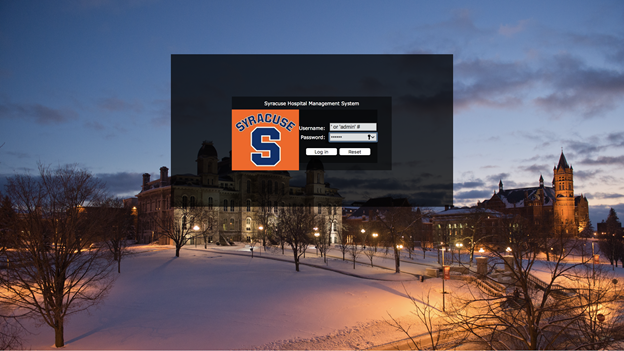
\includegraphics[width=\textwidth]{sp/sp1.png}
    \caption{Login with malicious input}
    \label{fig:s1}
\end{figure}
 
Click \emph{login} and see what will happen.
\begin{figure}[H]
    \centering
    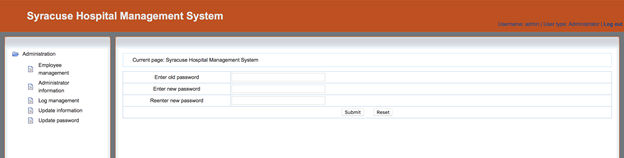
\includegraphics[width=\textwidth]{sp/sp2.png}
    \caption{Login success}
    \label{fig:s2}
\end{figure}

\subsubsection{Countermeasure}
A most common countermeasure of SQL injection is ‘prepared statement’. It means to create a query format with question signs. When a query request is sent to database, we replace the question signs in the format with actual data. Whatever we write will be treated as data, rather than  a part of the query conditions. Luckily, there is such method provided in JAVA, we just have to use provided class to achieve the countermeasure. Here is the code.
\begin{figure}[H]
    \centering
    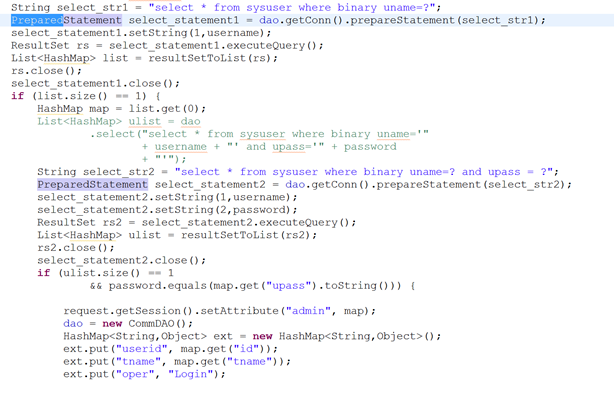
\includegraphics[width=\textwidth]{sp/sp3.png}
    \caption{Prepared Statement}
    \label{fig:s3}
\end{figure}
 
After applying prepared statement method, let’s try to repeat the attack. Here is the result.
\begin{figure}[H]
    \centering
    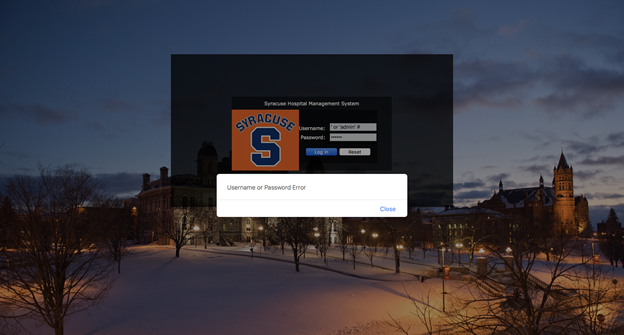
\includegraphics[width=\textwidth]{sp/sp4.png}
    \caption{Can't login}
    \label{fig:s4}
\end{figure}
 
As we can see, the attacker is unable to login as administrator now! SQL injection attack is prevented.

\subsection{CSRF attack}
\subsubsection{Introduction}
Cross-site request forgery, is a type of malicious exploit of a website where unauthorized commands are transmitted from a valid user that the target web application trusts. There are many ways in which a malicious website can transmit such commands. With a little help of social engineering (such as sending a link via email or chat), the attacker can lead the victim to access the malicious website, which may contains specially-crafted image tags, hidden forms, and JavaScript XMLHttpRequests, to send the unauthorized commands.
\subsubsection{Attack Simulation}
With CSRF attack, an attacker may trick the victim into executing actions of the attacker's choosing, without the victim approval. If the victim is a normal user, a successful CSRF attack can force the user to perform state changing requests like transferring funds, changing their email address, and so forth. If the victim is an administrative account, CSRF can compromise the entire target web application.

In our case, we write a malicious website to mock the behaviour of the attacker. After the victim login to the system, the victim access the malicious page and click submit. 
\begin{figure}[H]
    \centering
    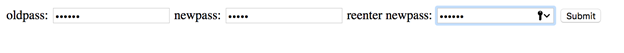
\includegraphics[width=\textwidth]{sp/sp5.png}
    \caption{malicious website mock}
    \label{fig:s5}
\end{figure}
As a result, the victim’s password has been modified.
\begin{figure}[H]
    \centering
    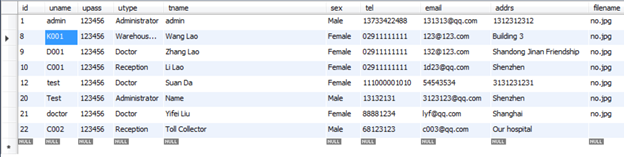
\includegraphics[width=\textwidth]{sp/sp6.png}
    \caption{Before CSRF attack}
    \label{fig:s6}
\end{figure}
\begin{figure}[H]
    \centering
    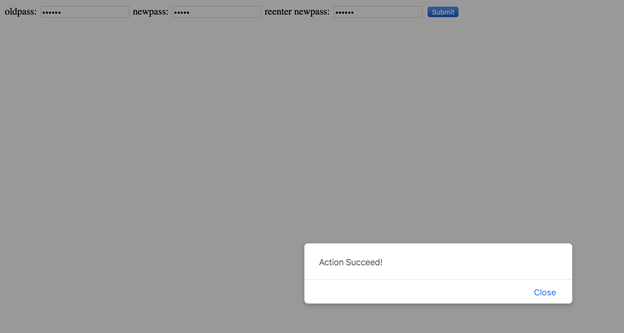
\includegraphics[width=\textwidth]{sp/sp7.png}
    \caption{modify password success}
    \label{fig:s7}
\end{figure}
\begin{figure}[H]
    \centering
    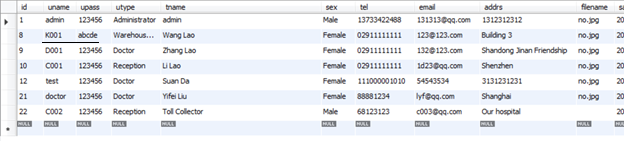
\includegraphics[width=\textwidth]{sp/sp8.png}
    \caption{After CSRF attack, the password has beem modified}
    \label{fig:s8}
\end{figure}
\subsubsection{Countermeasure}


A practical countermeasure against CSRF is to ensure the request has the same origin with the web application domain. The referrer header, which can enable the new web page to see where the request originated, is a ideal target to verify whether the origin of request matches the target origin or not.  Since the Referrer header can be only set by the browser, checking the Referrer header becomes a commonly used method of preventing CSRF. 

In our case, we implement the Referrer header checking like the following Figure \ref{fig:s9}:
\begin{figure}[H]
    \centering
    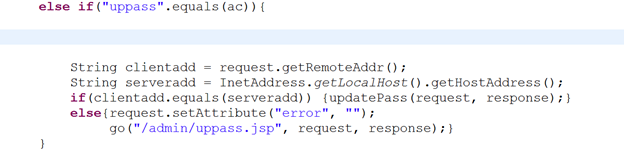
\includegraphics[width=\textwidth]{sp/sp9.png}
    \caption{CSRF countermeasure}
    \label{fig:s9}
\end{figure}
After enabling the countermeasure, we can observe the forged request from the malicious website has been blocked.
\begin{figure}[H]
    \centering
    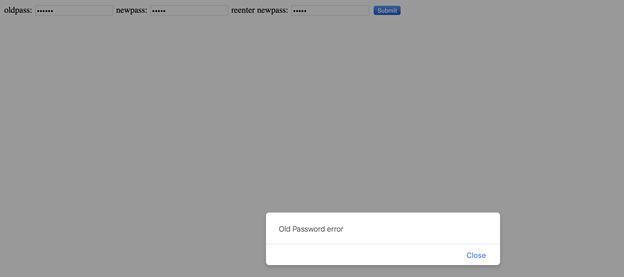
\includegraphics[width=\textwidth]{sp/sp10.png}
    \caption{Unauthorized request has been blocked}
    \label{fig:s10}
\end{figure}
\subsection{XSS attack}
\subsubsection{Introduction}
Cross-Site Scripting (XSS) attacks are a type of injection, in which malicious scripts are injected into otherwise benign and trusted web sites. XSS attacks occur when an attacker uses a web application to send malicious code, generally in the form of a browser side script, to a different end user. Flaws that allow these attacks to succeed are quite widespread and occur anywhere a web application uses input from a user within the output it generates without validating or encoding it.

\subsubsection{Attack Simulation}
An attacker can use XSS to send a malicious script to an unsuspecting user. The end user’s browser has no way to know that the script should not be trusted and will execute the script. Because it thinks the script came from a trusted source, the malicious script can access any cookies, session tokens, or other sensitive information retained by the browser and used with that site. These scripts can even rewrite the content of the HTML page. 

Here is an example to show how a malicious script is inserted to our website. We modify the full name of an employee to be a script. 
\begin{figure}[H]
    \centering
    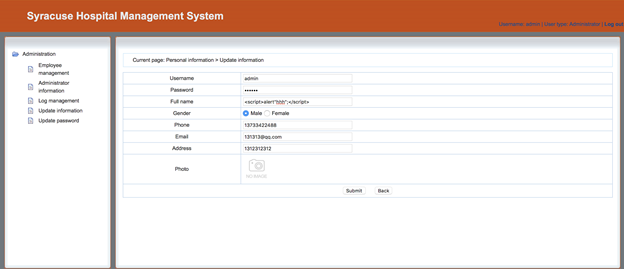
\includegraphics[width=\textwidth]{sp/sp11.png}
    \caption{Input with script}
    \label{fig:s11}
\end{figure}
 
Then we let the administrator login, and visit employee information page in to see what will happen.
\begin{figure}[H]
    \centering
    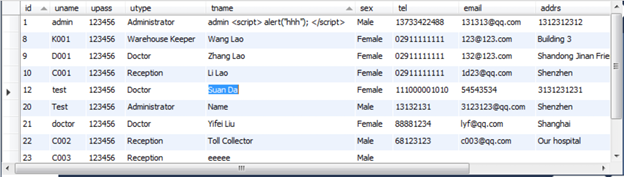
\includegraphics[width=\textwidth]{sp/sp12.png}
    \caption{Improper input has been submitted}
    \label{fig:s12}
\end{figure} 
As we can see in Figure \ref{fig:s13}, there is an alert box shown in the page. It means that administrator’s username and password information will be stolen by the attacker, if we change the content of the script. Therefore, our website is a potential victim of XSS attack
\begin{figure}[H]
    \centering
    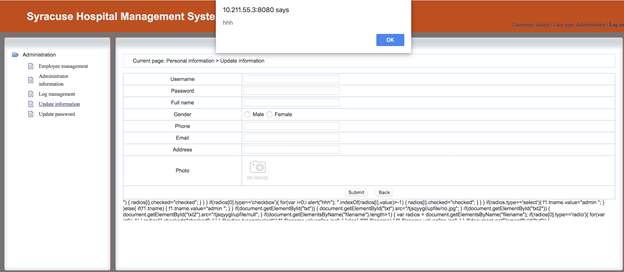
\includegraphics[width=\textwidth]{sp/sp13.png}
    \caption{Alert box}
    \label{fig:s13}
\end{figure} 

\subsubsection{Countermeasure}
To prevent this attack what we have to do is to remove or replace these sensitive characters or words. For example, we can replace $<$ and $>$ with \lbrack{} and \rbrack{} . As a result, the original script won’t be executed, because the string will never be treated as a script again.
 
Figure \ref{fig:s14} is how we implement it.
\begin{figure}[H]
    \centering
    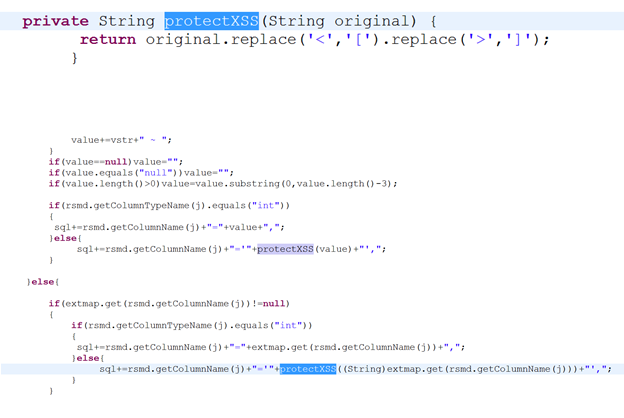
\includegraphics[width=\textwidth]{sp/sp14.png}
    \caption{XSS countermeasure: Filtering}
    \label{fig:s14}
\end{figure}
 
Now we repeat the attack and let the administrator visit employee information page again. As we can see, the sensitive characters are replaced, therefore XSS attack is prevented.
\begin{figure}[H]
    \centering
    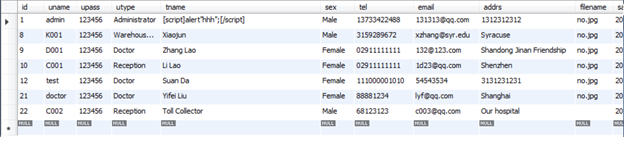
\includegraphics[width=\textwidth]{sp/sp15.png}
    \caption{Filtering works}
    \label{fig:s15}
\end{figure}

\subsection{Password Protection}
The protect of password is a critical block of the whole system. To achieve this, we implement two measures in our system.

\subsubsection{Hidden Password}
To prevent user’s password being pecked by others, we made it hidden when login or update password.
\begin{figure}[H]
    \centering
    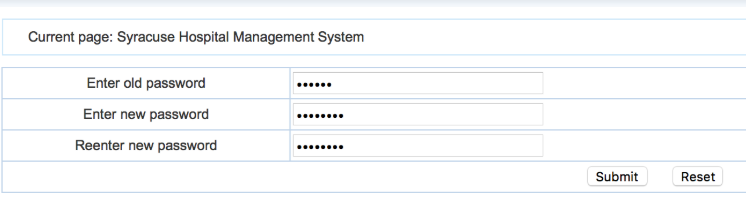
\includegraphics[width=\textwidth]{sp/sp01.PNG}
    \caption{Hidden Password}
    \label{fig:s01}
\end{figure}

\subsubsection{Hashed Password}
Instead of storing the plaintext of user password, the server only keep the hash value of the user password. With secure hash function, our system can provide the security promise that the attacker can not recover the user’s password even if the sensitive data in the server leaks. Thus the password our user is secured.

We have completed the password hash processing part in Java, however implementing hashed password involves several parts of system modules, including adding new account, modifying password and information, and log in part. As a result, there are still some work to be finished in the future.

\begin{figure}[H]
    \centering
    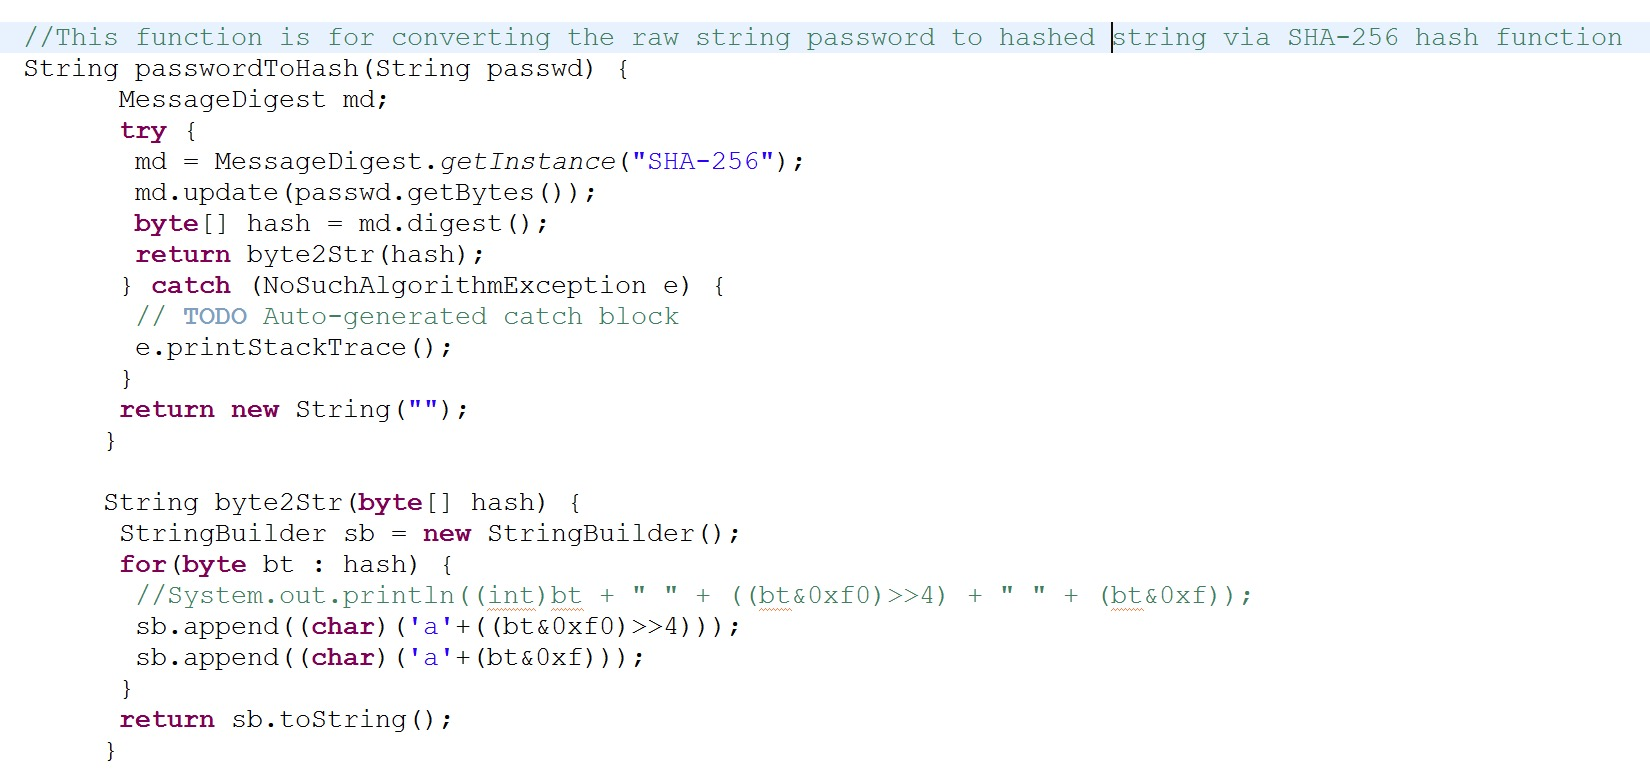
\includegraphics[width=\textwidth]{sp/sp02.jpg}
    \caption{Hashed Password}
    \label{fig:s02}
\end{figure}